\documentclass{classnotes}

\author{Jiaqi Wang}
\title{Discrete Structures}

\begin{document}

\maketitle

\tableofcontents
\newpage

\section{Sets}
\subsection{Functions}
\begin{proposition}
    Let $f: X \to Y$ and $g: Y \to Z$ be functions. Then
    \begin{enumerate}[label=(\roman*)]
        \item If $f,g$ are injective, then $g \circ f$ is also injective.
        \item If $f,g$ are surjective, then $g \circ f$ is also surjective.
        \item If $f,g$ are bijective, then $g \circ f$ is also bijective.
        \item For any function $f: X \to Y$, there exist a set $Z$, an injective 
            function $h: Z\to Y$, and a surjective function $g: X \to Z$, such that $f = h \circ g$
    \end{enumerate}
\end{proposition}
\subsection{Relations}
\begin{proposition}
    Let $R$ be a relation on a set $X$. Then
    \begin{enumerate}
        \item $R$ is reflexive if and only if $\Delta_X \subseteq R$. 
        \item $R$ is symmetric if and only if $R = R\inv$.
        \item $R$ is antisymmetric if and only if $R \cap R\inv \subseteq \Delta_X$.
        \item $R$ is transitive if and only if $R \circ R \subseteq R$.
    \end{enumerate}
    Where $\Delta_X = \{(x,x) \mid x \in X\}$.
\end{proposition}

\subsection{Orders}
\begin{proposition}
    Let $R$ be an order on a set $X$, Then $R \cup R\inv = X \times X$
\end{proposition}
\begin{definition}[Immediate predecessor]
    Let $(X, \sqsubseteq)$ be an ordered set. We say that an element $x \in X$ is an \emph{immediate predecessor} of an element $y \in X$ if
    \begin{itemize}
        \item $x \sqsubseteq y$, and
        \item there is no $t \in X$ such that $x \sqsubseteq t \sqsubseteq y$.
    \end{itemize}
\end{definition}
\begin{proposition}
    Let $(X,\sqsubseteq)$ be a finite-ordered set and let $\lhd$ be the corresponding immediate predecessor relation.
    Then for any two elements $x,y \in X, x \sqsubseteq y$ holds if and only if there exists elements $x_1,\dots,x_k \in X$
    such that $x \lhd x_1 \lhd \dots \lhd x_k \lhd y$ (possibly $k=0$, i.e. we may also have $x \lhd y$).
\end{proposition}

\begin{theorem}[Linear extension]
    Let $(X,\sqsubseteq)$ be a finite-poset. Then there exists a linear ordering $\le$ on $X$ such that $x \sqsubseteq y \implies x \le y$.
    The order $\le$ is called a \emph{linear extension} of $\sqsubseteq$.
\end{theorem}

\begin{definition}[Minimal/Maximal element]
    Let $(X,\sqsubseteq)$ be an ordered set. An element $a \in X$ is called a \emph{minimal element} if there is no $x \in X$ such that $x \sqsubseteq a$ and $x \ne a$.
    An element $b \in X$ is called a \emph{maximal element} if there is no $y \in X$ such that $b \sqsubseteq y$ and $b \ne y$.
\end{definition}

\begin{theorem}
    Every finite partially ordered set has at least one minimal element.
\end{theorem}

\begin{definition}[Smallet/Largest element]
    Let $(X,\sqsubseteq)$ be an ordered set. An element $a \in X$ is called a \emph{smallest element} if $\forall x \in X [a \sqsubseteq x]$.
    An element $b \in X$ is called a \emph{largest element} if $\forall y \in X [y \sqsubseteq b]$.
\end{definition}

\begin{definition}[Embedding]
    Let $(X,\sqsubseteq)$ and $(X^\prime,\sqsubseteq^\prime)$ be two ordered sets. A mapping $f: X \to X^\prime$ is called an \emph{embedding}
    of $(X,\sqsubseteq)$ into $(X^\prime,\sqsubseteq^\prime)$ if the following conditions hold:
    \begin{enumerate}[label=(\roman*)]
        \item $f$ is injective
        \item $\forall x,y \in X [x \sqsubseteq y \iff f(x) \sqsubseteq^\prime f(y)]$
    \end{enumerate}
\end{definition}

\begin{definition}[Isomorhpism]
    A surjective embedding is called an \emph{isomorphism}.
\end{definition}

\begin{theorem}
    For every ordered set $(X,\sqsubseteq)$ there exists an embedding into the ordered set $(\mathcal P(X),\subseteq)$
\end{theorem}

\begin{definition}
    A set $A \subseteq X$ is called \emph{independent} in $(X, \sqsubseteq)$ if we never have $x \sqsubseteq y$ for two
    distinct elements $x,y \in A$. It is also referred to as an \emph{antichain}.
\end{definition}

\begin{remark}
    The set of all minimal elements in $(X,\sqsubseteq)$ is independeent.
\end{remark}

\begin{definition}
    A set $A \subseteq X$ is called a \emph{chain} in $(X,\sqsubseteq)$ if for any two elements $x,y \in A$ we have $x \sqsubseteq y$ or $y \sqsubseteq x$.
\end{definition}

\begin{theorem}
    Let $(X,\sqsubseteq)$ be a poset and $\alpha$ be the maximum size of an independent set in $X$ and $\omega$ be the maximum size of a chain in $X$. 
    Then $\alpha \cdot \omega \ge |X|$.
\end{theorem}

\begin{theorem}[Erd\"os - Szekeres]
    Let $n \in \mathbb N$. Then every sequence of $n^2+1$ distinct real numbers contains a monotone subsequence of length $n+1$.
\end{theorem}

\section{Counting}

\subsection{functions}
\begin{proposition}
    Let $|N| =n, |M| = m$. Then number of all possible mappings $f: N \to M$ is $m^n$.
\end{proposition}

\begin{proposition}
    An  $n$-element set $X$ has exactly $2^n$ subsets.
\end{proposition}

\begin{proposition}
    Let $n \ge 1$. Each $n$-element set has exactly $2^{n-1}$ subsets of an odd size and exactly $2^{n-1}$ subsets of an even size.
\end{proposition}

\begin{proposition}
    For given numbers $n,m \ge 0$, there exists exactly
    $$m(m-1)\dots(m-n+1) = \prod_{i=0}^{n-1}(m-i)$$
    injective mappings $f: \{1,2,\dots,n\} \to \{1,2,\dots,m\}$.
\end{proposition}

\subsection{Permutations}
\begin{definition}[Permutation]
    $|\sym_n| = n!$
\end{definition}

\subsection{Binomial coefficients}
\begin{proposition}
    For any finite set $X$, the number of all $k$-element subsets equals $\binom{|X|}{k}$.
\end{proposition}

\begin{proposition}[Balls and bins]
    $\binom{m+r-1}{r-1}$
\end{proposition}

\subsection{Include-exclude principle}


\section{Graphs}
\subsection{Graphs}
\begin{definition}[Isomorhpism]
    Two graphs $G=(V,E)$ and $G^\prime = (V^\prime,E^\prime)$ are called \emph{isomorphic} if there exists a bijection $f: V \to V^\prime$ such that
    $\forall x,y \in V, x \ne y [\{x,y\} \in E \iff \{f(x),f(y)\} \in E^\prime]$

    Such a bijection $f$ is called an \emph{isomorphism} from $G$ to $G^\prime$.
\end{definition}

\begin{theorem}[Counting graphs]
    Let $V=\{1,2,\dots,n\}$. There are $2^{\binom{n}{2}}$ possible graphs.
\end{theorem}

\subsection{Subgraphs}
\begin{definition}[Subgraph]
    A graph $G^\prime = (V^\prime,E^\prime)$ is a \emph{subgraph} of $G=(V,E)$ if $V^\prime \subseteq V$ and $E^\prime \subseteq E$.
\end{definition}

\begin{definition}[Induced subgraph]
    A graph $G^\prime = (V^\prime,E^\prime)$ is an \emph{induced subgraph} of $G=(V,E)$ if $V^\prime \subseteq V$ and $E^\prime = \{\{x,y\} \in E \mid x,y \in V^\prime\}$.
\end{definition}

\subsection{Common graphs}
\subsubsection*{Complete graphs}
\begin{definition}[Complete graph]
    A graph $G=(V,E)$ is a \emph{complete graph} if $\forall x,y \in V, x \ne y [\{x,y\} \in E]$.
\end{definition}
\begin{proposition}
    Let $V = \{1,2,\dots,n\}$ and $K_n$ be the complete graph on $V$. Then $K_n$ has $\binom{n}{2}$ edges.
\end{proposition}

\subsubsection*{Star graphs}
\begin{definition}[Star graph]
    A graph $G=(V,E)$ is a \emph{star graph} if $V=\{u\}\cup\{v_1,\dots,v_n\}$ and $E = \{\{u,v_j\} \mid j = 1,2,\dots,n\}$.
\end{definition}
\begin{proposition}
    Let $V = \{1,2,\dots,n\}$ and $S_n$ be the star graph on $V$. Then $S_n$ has $n-1$ edges.
\end{proposition}

\subsubsection*{Complete bipartite graphs}
\begin{definition}[Complete bipartite graph]
    A graph $G=(V,E)$ is a \emph{complete bipartite graph} if $V=V_1 \cup V_2$ and $E = \{\{x,y\} \mid x \in V_1, y \in V_2\}$.
\end{definition}
\begin{proposition}
    Let $V_1 = \{1,2,\dots,n\}$ and $V_2 = \{n+1,n+2,\dots,n+m\}$ and $K_{n,m}$ be the complete bipartite graph on $V_1 \cup V_2$. Then $K_{n,m}$ has $n \cdot m$ edges.
\end{proposition}

\subsubsection*{Paths}
\begin{definition}[Path]
    A graph $G=(V,E)$ is a \emph{path} if $V=\{v_1,v_2,\dots,v_n\}$ and $E = \{\{v_i,v_{i+1}\} \mid i = 1,2,\dots,n-1\}$.
\end{definition}
\begin{proposition}
    Let $V = \{1,2,\dots,n\}$ and $P_n$ be the path on $V$. Then $P_n$ has $n-1$ edges.
\end{proposition}

\subsubsection*{Cycles}
\begin{definition}[Cycle]
    A graph $G=(V,E)$ is a \emph{cycle} if $V=\{v_1,v_2,\dots,v_n\}$ and $E = \{\{v_i,v_{i+1}\} \mid i = 1,2,\dots,n-1\} \cup \{\{v_n,v_1\}\}$.
\end{definition}
\begin{proposition}
    Let $V = \{1,2,\dots,n\}$ and $C_n$ be the cycle on $V$. Then $C_n$ has $n$ edges.
\end{proposition}

\subsection{Walks}
\begin{definition}[Walk]
    A \emph{walk} in a graph $G=(V,E)$ is a sequence of vertices $v_1,v_2,\dots,v_n$ such that $\forall i \in \{1,2,\dots,n-1\} [\{v_i,v_{i+1}\} \in E]$.

    Another definition is that a walk is a sequence of edges $e_1,e_2,\dots,e_n$ such that $\forall i \in \{1,2,\dots,n-1\} [e_i = \{v_i,v_{i+1}\}]$.
\end{definition}

\subsection{Connected and Components}
\begin{definition}[Connected]
    A graph $G=(V,E)$ is \emph{connected} if $\forall x,y \in V \left[\exists \text{ a walk from }x \text{ to }y\right]$.
\end{definition}

\begin{definition}[Component]
    The components of a graph $G$ are the equivalence classes defined by the relation $~$ on the set $V(G)$, where $x~y \iff \exists \text{a walk from $x$ to $y$ in $G$} $
\end{definition}

\begin{theorem}
    Any graph $G=(V,E)$ where each vertex $v\in V$ has $\deg_G(v) \ge \frac{n-1}{2}$ is connected, where $n = |V|$.
\end{theorem}

\subsection{Graph distance}
\begin{definition}[Distance]
    The \emph{distance} between two vertices $x$ and $y$ in a graph $G$ is the length of the shortest walk from $x$ to $y$ in $G$.
\end{definition}

\begin{theorem}
    Let $G=(V,E)$ with vertex set $V=\{v_1,\dots,v_n\}$ be a graph and let $A$ be its adjacency matrix. Let $a_{i,j}^k$ denote the element of $A^k$ at position
    $(i,j)$. Then $a_{i,j}^k$ is the number of walks of length $k$ from $v_i$ to $v_j$.
\end{theorem}

\subsection{Degree sequence}
\begin{definition}[Degree sequence]
    The \emph{degree sequence} of a graph $G=(V,E)$ is the sequence of degrees of the vertices of $G$.

    The order doesn't matter. Generally, we sort the sequence in non-decreasing order.
\end{definition}
\begin{example}
    The degree sequence of the graph $G$ is $(1,2,2,4,4,4,4,4)$.
    \begin{center}
        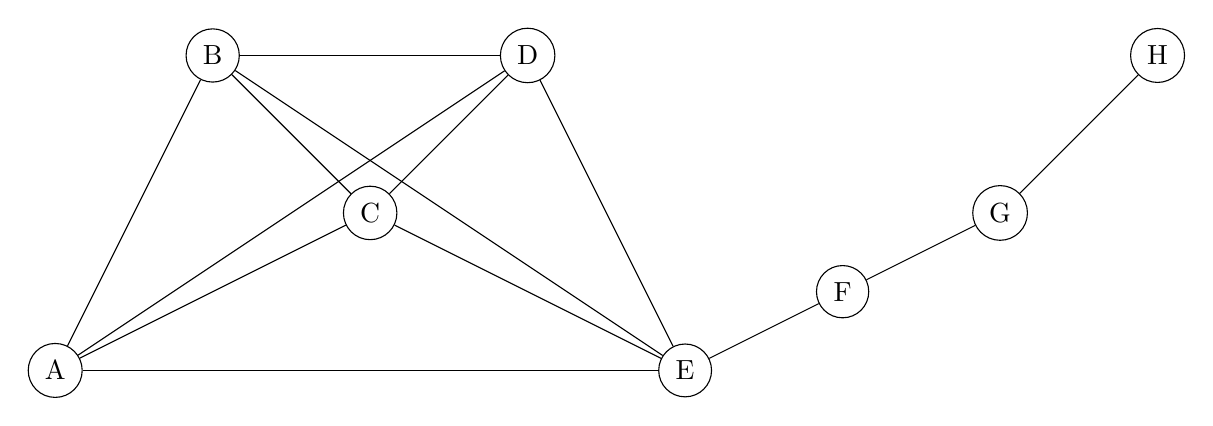
\begin{tikzpicture}
            \node[shape=circle,draw=black] (A) at (0,0) {A};
            \node[shape=circle,draw=black] (B) at (2,4) {B};
            \node[shape=circle,draw=black] (C) at (4,2) {C};
            \node[shape=circle,draw=black] (D) at (6,4) {D};
            \node[shape=circle,draw=black] (E) at (8,0) {E};
            \node[shape=circle,draw=black] (F) at (10,1) {F};
            \node[shape=circle,draw=black] (G) at (12,2) {G};
            \node[shape=circle,draw=black] (H) at (14,4) {H};

            \path [-] (A) edge (B);
            \path [-] (A) edge (C);
            \path [-] (A) edge (D);
            \path [-] (A) edge (E);
            \path [-] (B) edge (C);
            \path [-] (B) edge (D);
            \path [-] (B) edge (E);
            \path [-] (C) edge (D);
            \path [-] (C) edge (E);
            \path [-] (D) edge (E);
            \path [-] (E) edge (F);
            \path [-] (F) edge (G);
            \path [-] (G) edge (H);
        \end{tikzpicture}
    \end{center}
\end{example}
\begin{example}
    A path of length $n$ has degree sequence $(2,1,1,\dots,1,2)$.
\end{example}
\begin{example}
    A cycle of length $n$ has degree sequence $(2,2,\dots,2)$.
\end{example}
\begin{example}
    A complete graph of $n$ vertices has degree sequence $(n-1,n-1,\dots,n-1)$.
\end{example}
\begin{example}
    A complete bipartite graph $K_{n,m}$ has degree sequence $(m,m,\dots,m,n,n,\dots,n)$.
\end{example}

\begin{remark}
    A sequence of non-negative integers is a degree sequence of some graph if and only if the sum of the integers is even.
\end{remark}

\begin{lemma}[Hankshake lemma]
    For any graph $G=(V,E)$ the number of vertices of odd degree is even.
\end{lemma}

\begin{theorem}
    Let $D = (d_1,\dots,d_n)$ be a sequence of natural numbers, for $n > 1$, where $d_1 \le d_2 \le \dots \le d_n \le n_1$ and let $D^\prime$ denote the
    sequence $(d_1^\prime,\dots,d_{n-1}^\prime)$ where 
    $$d_i^\prime = \begin{cases}d_i &\text{ for } i < n-d_n \\ d_i - 1 &\text{ for }i\ge n-d_n\end{cases}$$
    Then $D$ is a degree sequence if and only if $D^\prime$ is a degree sequence.
\end{theorem}

\subsection{Eulerian graphs}
\begin{definition}[Closed Eulerian tour]
    A closed walk containing all the vertices and edges, and each edge exactly once, is called a \emph{closed Eulerian tour}.
\end{definition}

\begin{definition}[Eulerian graph]
    A graph $G=(V,E)$ is \emph{Eulerian} if it has a closed Eulerian tour.
\end{definition}

\begin{theorem}
    A graph $G=(V,E)$ is Eulerian if and only if $G$ is connected and each vertex has even degree.
\end{theorem}

\subsection{Hamiltonian cycle}
\begin{definition}[Hamiltonian cycle]
    A \emph{Hamiltonian cycle} is a cycle that contains all the vertices of a graph.
\end{definition}

\subsection{Graph operations}
\begin{definition}[Graph operations]
    Let $G=(V,E)$ be a graph
    \begin{enumerate}
        \item Edge deletion: $G-e = (V,E\setminus\{e\})$, where $e \in E$.
        \item Edge insertion: $G+e = (V,E \cup \{e\})$, where $e \in \binom{V}{2}\setminus E$
        \item Vertex deletion: $G-v = (V-\{v\},\{e \in E \mid v \in e\})$, where $v \in V$.
        \item Edge subdivision: $G\%e = (V\cup\{z\},(E \setminus \{\{x,y\}\}) \cup \{\{x,z\},\{z,y\}\})$ where $e = \{x,y\} \in E$ and $z \notin V$.
        % \item Edge contraction: $G/e = (V^\prime,E^\prime)$ where $V^\prime = V-\{x,y\} \cup \{z\}$ and $E^\prime = (E-\{e\}) \cup \{\{x,z\},\{y,z\}\}$.
    \end{enumerate}
\end{definition}

\subsection{K-vertex-connectivity}
\begin{definition}
    A graph $G$ is called \emph{k-vertex-connected} if $|V(G)| \ge k+1$ and $G-v$ is connected for every $v \in V(G)$.
    Often we say $G$ is $k$-connected.
\end{definition}
\begin{example}
    $K_n$ is $(n-1)$-connected.
\end{example}

\begin{theorem}
    A graph $G=(V,E)$ is 2-connected if and only if for any two vertices $v,w \in V$, there exists a cycle containing $v$ and $w$. 
\end{theorem}

\section{Trees}
\subsection{Definition}
\begin{definition}[Tree]
    A \emph{tree} is a connected graph with no cycles.
\end{definition}

\begin{theorem}
    For a non-empty graph $G=(V,E)$, the following are equivalent:
    \begin{enumerate}
        \item The graph $G$ is a tree.
        \item For any two distinct vertices $u,v \in V$, there is a unique path from $u$ to $v$. \hfill (unique paths)
        \item The graph $G$ is connected and $\forall e \in E, G-e$ is disconnected. \hfill (minimal connected graph)
        \item The graph $G$ is acyclic and $\forall e \in \binom{V}{2}\setminus E, G+e$ contains a cycle. \hfill (maximal acyclic graph)
        \item $G$ is connected and $|V| = |E|+1$. \hfill (Euler's formula)
    \end{enumerate}
\end{theorem}

\subsection{Induction on trees}
\begin{lemma}[end-vertex]
    Every tree with at least two vertices has at least two leaves.
\end{lemma}
\begin{lemma}[tree-growing]
    Let $G$ be a graph and $v$ be a leaf in $G$. Then $G-v$ is a tree.
\end{lemma}

\subsection{Rooted trees}
\begin{definition}[Rooted tree]
    A \emph{rooted tree} is a pair $(T,r)$  where $T$ is a tree and $r \in V(T)$ is a distinguished vertex of $T$ called \emph{the root}.

    A node $u$ in a rooted tree $T$ may have a:
    \begin{enumerate}
        \item parent: the unique vertex $v \in V(T)$ such that $\{u,v\} \in E(T)$ and $v$ lies on the unique path from $u$ to $r$,
        \item ancestor: a vertex $v \in V(T)$ such that $v$ lies on the unique path from $u$ to $r$,
        \item child: a vertex $v \in V(T)$ where $u$ is the parent of $v$,
        \item descendant: a vertex $v \in V(T)$ where $u$ is an ancestor of $v$,
    \end{enumerate}
\end{definition}

\subsection{Subtree}
\begin{definition}[Subtree]
    The \emph{subtree rooted at $v \in V(T)$} in a rooted tree is the induced subgraph defined by all vertices that are descendants of $v$, rooted at $v$.
\end{definition}

\subsection{Binary trees}
\begin{definition}[Binary tree]
    A \emph{binary tree} is a rooted tree where each node has at most two children.
\end{definition}

\begin{definition}[Strict binary tree]
    A \emph{strict binary tree} is a rooted tree where each node has exactly zero or two children.
\end{definition}

\begin{lemma}
    A strict binary tree with $n$ vertices has $\frac{n-1}{2}$ internal vertices.
\end{lemma}

\subsection{Ear decomposition}
\begin{lemma}
    Let $G = (V,E)$ be a 2-connected graph, then
    \begin{enumerate}
        \item $G\%e$ is 2-connected graph, where $e \in E$
        \item $G+e$ is a 2 connected graph, where $e \in \binom{V}{2}\setminus E$
    \end{enumerate}
\end{lemma}

\begin{proposition}
    Any 2-connected graph $G=(V,E)$ can be connected from $K_3$ by a sequence of edges subdivisions and edge additions.
\end{proposition}

\begin{definition}[Ear decomposition]
    An \emph{ear decomposition} of a graph $G=(V,E)$ is a sequence of subgraphs $G_0,G_1,\dots,G_k$ of $G$ such that
    \begin{enumerate}
        \item $G_0$ is a cycle,
        \item $G_k = G$,
        \item $G_i = G_{i-1}\%e_i$ or $G_i = G_{i-1}+e_i$ for $i = 1,2,\dots,k$.
    \end{enumerate}
\end{definition}

\begin{theorem}
    Any 2-connected graph $G$ has an ear decomposition.
\end{theorem}

\section{Directed Graphs}
\subsection{Definition}
\begin{definition}[Directeed graph]
    A directed graph $G$ is an order pari $(V,E)$, where $V$ is some set of elements and $E \subseteq V \times V$.

    A \emph{directed edge} $e = (u,v)$, called an edge from $u$ to $v$, has \emph{head} $v$ and \emph{tail} $u$.

    The \emph{indegree $\deg_G^+(v)$} of a vertex $v$ is the number of edges having $v$ as head. The \emph{outdegree $\deg_G^-(v)$} is the number of
    edges having $v$ as tail.
\end{definition}

\subsection{Connectedness}
\begin{definition}[Symmetrization]
    The \emph{symmetrization} of a directed graph $G=(V,E)$ is the undirected graph $\sym(G) = (V,\overline{E})$ where $\overline{E} = \{ \{u,v\} \mid (u,v) \in E \lor (v,u) \in E \}$
\end{definition}

\begin{definition}[Weakly connected]
    A directed graph $G$ is called \emph{weakly connected} if its symmetrization $\sym(G)$ is connected.
\end{definition}

\begin{definition}[Strongly connected]
    A directed graph $G$ is called \emph{strongly connected} if for every two vertices $u,v \in V$ there is a directed path from $u$ to $v$ and a directed path from $v$ to $u$.
\end{definition}

\begin{definition}[Weakly conneccted components]
    \emph{Weakly connected components} of a directed graph $G$ are the equivalence classes defined by the relation $~$ on the set $V(G)$, where $x~y \iff \exists \text{a walk from $x$ to $y$ in $\sym(G)$} $
\end{definition}

\begin{definition}[Strongly connected components]
    \emph{Strongly connected components} of a directed graph $G$ are the equivalence classes defined by the relation $~$ on the set $V(G)$, where $x~y \iff \exists \text{a directed walk from $x$ to $y$ and from $y$ to $x$ in $G$} $
\end{definition}

\subsection{Eulerian directed graphs}
\begin{definition}[Eulerian directed tour]
    A closed directed walk containing all the vertices and edges, and each edge exactly once is an \emph{Eulerian directed tour}.
\end{definition}

\begin{definition}[Eulerian directed graph]
    A directed graph $G$ is \emph{Eulerian} if it has an Eulerian directed tour.
\end{definition}

\begin{theorem}
    A directed graph is Eulerian if and only if its symmetrization is connected and $\deg^+(v) = \deg^-(v)$ for all $v \in V$.
\end{theorem}

\subsection{De Bruijn Graphs}
\begin{lemma}
    Every vertex $v$ in a De Bruijn graph has $\deg^+(v)=\deg^-(v)$.
\end{lemma}
\begin{lemma}
    For any De Bruijn graph $G$, $\sym(G)$ is connected.
\end{lemma}

\subsection{Directed acyclic graphs}
\begin{definition}[Directed acyclic graph]
    A \emph{directed acyclic graph} is a directed graph with no directed cycles.
\end{definition}

\begin{definition}[Source]
    A \emph{source} in a directed graph $G$ is a vertex $v$ such that $\deg^+(v) = 0$.
\end{definition}
\begin{definition}[Sink]
    A \emph{sink} in a directed graph $G$ is a vertex $v$ such that $\deg^-(v) = 0$.
\end{definition}

\begin{theorem}
    Every (finite) DAG $G = (V,E)$ has at least one sink.
\end{theorem}

\section{Planar Graphs}
\subsection{Definitions}
\begin{definition}[Planar graph]
    A \emph{planar graph} is a graph that can be drawn in the plane without any edges crossing.
\end{definition}

\begin{definition}[Arc]
    An \emph{arc} is an injective continuous function $\gamma: [0,1] \to \mathbb{R}^2$.
\end{definition}

\begin{definition}[Drawing]
    A \emph{drawing} of  a graph $G=(V,E)$ is an assignment:
    \begin{itemize}
        \item to every vertex $v \in V$ a point $b(v)$ of the plane
        \item to every edge $e = \{u,v\} \in E$, assign an arc $a(e)$ in the plane with endpoints $b(u)$ and $b(v)$
    \end{itemize}
    such that
    \begin{itemize}
        \item the mapping $b$ is injective
        \item no point $b(v)$ lies on any of the arcs $a(e)$ unless it is an endpoint of that arc
    \end{itemize}
\end{definition}

\begin{definition}[Topological graph]
    A \emph{topological graph} is a graph together with a drawing.
\end{definition}

\subsection{Faces}
\begin{definition}[Face]
    A \emph{face} of a drawing of a graph $G$ is a maximal connected subset of the plane whose boundary consists of arcs $a(e)$ for edges $e \in E$.
\end{definition}

\begin{definition}[Jordan curve]
    A \emph{Jordan curve} is an arc whose endpoints coincide.
\end{definition}

\begin{theorem}
    Any Jordan curve $k$ divides the plane into exactly two connected parts, the "interior" and the "exterior" of $k$, and $k$ is the boundary of both the interior and exterior.
\end{theorem}

\subsection{Planar graphs}
\begin{proposition}
    $K_1,K_2,K_3,K_4$ are planar.

    $K_5$ is not planar.
\end{proposition}
\begin{proposition}
    $K_{3,3}$ is not planar
\end{proposition}

\begin{theorem}[Kuratowski's theorem]
    A graph $G$ is planar if and only if it has no subgraph isomorphic to a subdivision of $K_{3,3}$ or to a subdivision of $K_5$
\end{theorem}

\subsection{Properties of planar graphs}
\begin{theorem}[Euler's formula]
    Let $G=(V,E)$ be a connected planar graph and let $f$ be the number of faces of some planar drawing of $G$. Then we have 
    $$|V|-|E|+f=2$$
\end{theorem}

\begin{theorem}
    Let $G=(V,E)$ be a planar graph with at least 3 vertices. Then
    $$|E| \le 3|V| - 6.$$
\end{theorem}

\begin{corollary}
    Every planar graph contains a vertex of degree at most 5.
\end{corollary}

\subsection{Coloring maps}
\begin{definition}
    A mapping $c: V \to \{1,2,\dots,k\}$ is called a \emph{coloring} of a graph $G=(V,E)$ if $c(u) \ne c(v)$ for every edge $\{u,v\} \in E$.
\end{definition}

\begin{definition}[Chromatic number]
    The \emph{chromatic number}, denoted by $\chi(G)$, of a graph $G$ is the smallest $k$ such that $G$ has a coloring $c: V \to \{1,2,\dots,k\}$.
\end{definition}

\begin{example}
    $\chi(K_n) = n$.
\end{example}
\begin{example}
    $\chi(K_{n,m}) = 2$.
\end{example}
\begin{example}
    $\chi(C_n) = \begin{cases} 2 &\text{ if } n \text{ even}\\ 3 &\text{ if } n \text{ odd}\end{cases}. $
\end{example}
\begin{example}
    $\chi(P_n) = 2$.
\end{example}
\begin{example}
    $\chi(T_n) = 2$.
\end{example}

\begin{theorem}
    Any planar graph satisfies $\chi(G) \le 4$.
\end{theorem}

\section{Double Counting}
\subsection{Double Counting}
\begin{theorem}
    If $G=(V,E)$ is a triangle-free graph with $n$ vertices, then $G$ has at most $\frac{n^2}{4}$ edges.
\end{theorem}
\begin{theorem}
    If $G=(V,E)$ is a n-vertex graph without a $K_{2,2}$ subgraph, then $G$ has at most $\frac{1}{2}(n^{\frac{3}{2}} +n)$ edges
\end{theorem}
\begin{proposition}
    Let $G=(V,E)$ be a graph with $n$ vertices and $m$ edges. 
    $$\sum_{v \in V} \deg(v) = 2 |E|.$$
\end{proposition}

\end{document}
